\section{Zielsetzung}
\label{sec:Zielsetzung}
In diesem Versuch soll zuerst die Zeitabhängigkeit der Amplitude und den effektiven Dämpfungswiderstand bestimmt werden. Bei dem aperiodischen Grenzfall tritt den Dämpfungswiderstand auf, der ebenfalls bestimmt werden soll. Als letztes wird die Frequenzabhängigkeit bei der Kondensatorspannung und bei der Phasenverschiebung ermittelt. 
\section{Theorie}
\label{sec:Theorie}
Ein LC-Schwingkreis besteht hauptsächlich aus einer Induktivität $L$ und eine Kapazität $C$. Das System enthält zwei Energiespeichern, bei dem die eingespeicherte Energiemenge zwischen den beiden hin und her ausgetauscht wird. Dabei wechselt der Strom $I(t)$ periodisch sein Vorzeichen. 
Bei einer ungedämpften Schwingung bleibt die Energiemenge erhalten, solange kein Element im Schaltkreis existiert, das Energie verbraucht. 

Es kommt zu einer gedämpften Schwingung erst wenn ein ohmscher Widerstand $R$ hinzugefügt wird und an diesem die elektrische Energie in Wärmeenergie umgesetzt wird. Damit ist $R$ als Dämpfungsfaktor anzusehen. Der Schwingkreis ist in der Abbildung \ref{fig:schwingkreisrcl} zu sehen und die einzelnen Spannungen, die über jeden Bauteil mit der Zeit abfallen. 
\begin{figure}[h!]
	\centering
	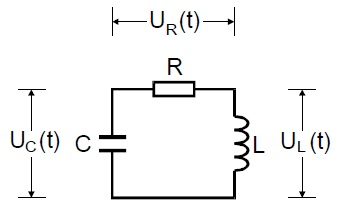
\includegraphics[width=0.7\linewidth]{SchwingkreisRCL}
	\caption{Aufbau eines RCL-Schwingkreises, \cite[1]{anleitung354}.}
	\label{fig:schwingkreisrcl}
\end{figure}
 
Nach der Maschenregel bzw. nach dem $2.$ Kirchhoff'schen Gesetz ist die Summe aller Spannungen gleich null und es gilt:
\begin{equation*}
U_{\text{R}}(t) + U_{\text{C}}(t) + U_{\text{L}}(t) = 0.
\end{equation*}
Jede Spannung wird durch den Strom $I$ ausgedrückt und es entspricht dann:
\begin{align*}
U_{\text{R}}(t) &= RI(t) \\
U_{\text{C}}(t) &= \frac{Q(t)}{C}
\end{align*} 
wobei $I = \frac{dQ}{dt}$ und:
\begin{equation*}
U_{\text{L}}(t) = L\dot{I}.
\end{equation*}
Es wird mit Hilfe den Umformungen für die Spannungen umgeschrieben und es ergibt sich eine Differentialgleichung $2.$ Ordnung:
\begin{equation*}
\ddot{I}(t) + \frac{R}{L}\dot{I}(t) + \frac{1}{LC}I(t) = 0.
\end{equation*}
Die Lösung der Differentialgleichung lautet dann:
\begin{equation}
\label{eq:DGL}
I(t) = e^{-2 \pi \mu t}(A_{1}e^{2i \pi \nu t}+A_{2}e^{-2i \pi \nu t}).
\end{equation}
Zur Vereinfachung werden bei der Lösung für die Differentialgleichung auch Abkürzungen verwendet, die lauten:
\begin{align}
\label{eq:Fallunterscheidung}
2 \pi \mu &= \frac{R}{2L} \\
2 \pi \nu &= \sqrt{\frac{1}{LC}-\frac{R^{2}}{4L^{2}}}.
\end{align}
Hier muss die Fallunterscheidung untersucht werden, weil die Form der Differentialgleichung von $\nu$ abhängt, also ob $\nu$ reell oder imaginär ist.
Es gilt also:
\begin{equation*}
\begin{cases}
\frac{1}{LC} > \frac{R^{2}}{4L^{2}}, & \text{reelle Lösung} \\
\frac{1}{LC} < \frac{R^{2}}{4L^{2}}, & \text{imaginäre Lösung}.
\end{cases}
\end{equation*}
Wenn der reelle Fall für die Formel \ref{eq:DGL} erfüllt ist, dann ergibt sich unter Benutzung der Eulerschen Formel für Cosinus das folgende Ergebnis:
\begin{equation}
\label{eq:reell}
I(t) = A_{0}e^{-2\pi\mu t}\text{cos}(2\pi\nu t+\eta).
\end{equation}
Das Ergebnis aus \ref{eq:reell} entspricht einer gedämpften Schwingung, die mit zunehmender Zeit exponentiellen gegen 0 geht. 
Die Schwingungsdauer ist gegeben als:
\begin{equation}
\label{eq:Schwingungsdauer}
T = \frac{1}{\nu}
\end{equation}
wobei $\nu$ die Frequenz darstellt.
Wenn für die Formel der Schwingungsdauer aus \ref{eq:Schwingungsdauer} $\nu$ mit der ersten Formel aus \ref{eq:Fallunterscheidung} ersetzt wird, dann ergibt sich die Abklingdauer, die einem Zeitraum entspricht, in dem die Amplitude auf einen bestimmten e-ten Teil abfällt:
\begin{equation*}
T_{\text{ex}} = \frac{1}{2 \pi \nu} = \frac{2L}{R}.
\end{equation*}
Für den Fall, dass $\nu$ imaginär ist, liegt die aperiodische Dämpfung vor, das bedeutet die Amplitude des Stroms $I(t)$ kann einen Extremwert erreichen oder es kann gegen null gehen. Dann gilt für die Lösung der Differentialgleichung aus \ref{eq:DGL}:
\begin{equation}
\label{eq:imaginär}
I(t) \propto e^{-(\frac{R}{2L}-\sqrt{\frac{R^{2}}{4L^{2}}-\frac{1}{LC}})t}.
\end{equation}
Es erfolgt nämlich den Spezialfall, wo $\nu = 0$ ist und es ergibt sich:
\begin{equation*}
\frac{1}{LC} = \frac{R_\text{ap}^{2}}{4L^{2}}.
\end{equation*}
Der Exponent bleibt in \ref{eq:imaginär} reell, und daraus folgt:
\begin{equation*}
I(t) = A \cdot e^{-{\frac{R}{2L}t}} = A \cdot e^{-\frac{t}{\sqrt{LC}}}.
\end{equation*}
Weil die Amplitude der Stroms $I(t)$ hier am schnellsten gegen 0 geht, ohne dabei zu schwingen, wird dieser Fall als aperiodischer Grenzfall bezeichnet.

In diesem Versuch wird der RLC-Schwingkreis zusätzlich unter dem Einfluss einer äußeren periodischen Kraft(Spannung) untersucht. Also es wird zusätzlich eine sinusförmige Wechselspannungsquelle hinzugefügt, die in der Abbildung \ref{fig:rlcw} zu sehen ist. 
\begin{figure}[h!]
	\centering
	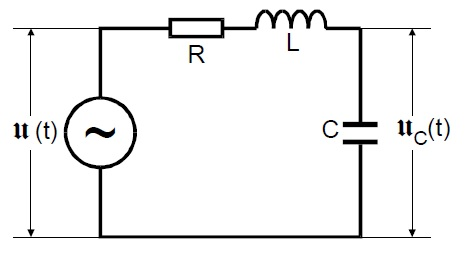
\includegraphics[width=0.7\linewidth]{content/RLCW}
	\caption{Aufbau eines RLC-Kreises bei erzwungenen Schwingungen,\cite[6]{anleitung354}}
	\label{fig:rlcw}
\end{figure}
In diesem Fall liegt eine inhomogene Differentialgleichung zweiter Ordnung vor, die aussieht wie:
\begin{equation}
\label{eq:inhDGL}
LC\ddot{U_\text{C}}(t) + RC\dot{U_\text{C}}(t) + U_\text{C}(t) = U_\text{0}e^{i\omega t}.
\end{equation}
Für die Differentialgleichung ergibt sich eine Lösung für die Spannung, die nach der Zeit abhängig ist:
\begin{equation}
\label{eq:inhLSG}
U(t) = \frac{U_{0}(1-LC\omega^{2}-i\omega RC)}{(1-LC\omega^{2})^{2}+\omega^{2}R^{2}C^{2}}.
\end{equation}
Für die Erhaltung der Formel bei der Phasenverschiebung wird bei der Formel \ref{eq:inhLSG} den imaginären und reellen Teil verglichen und daraus folgt:
\begin{equation}
\phi(\omega) = \text{arctan}\left(\frac{\text{Im}(U)}{\text{Re}(U)}\right) = \text{arctan}\left(\frac{-\omega RC}{1-LC\omega^{2}}\right).
\end{equation}
An dieser Stelle lässt sich die Abhängigkeit der Frequenz von der Phase zwischen Erreger- und Kondensatorspannung erkennen. Für kleine Frequenzen sind die beiden Spannungen in Phase und bei hoher Frequenz bleibt $U_\text{C}$ hinter $U_{0}$ um $\pi$ zurück.
An dieser Gleichung lässt sich auch noch erkennen, dass für Frequenzen, bei denen die Phasenverschiebung $\frac{\pi}{4}$ oder $\frac{3}{4}\pi$ beträgt, gilt also:
\begin{equation*}
\omega_{1,2} = \pm \frac{R}{2L} + \sqrt{\frac{R^{2}}{4L^{2}}+\frac{1}{LC}}
\end{equation*}
Die Spannung des Kondensators lässt sich auch in Abhängigkeit von der Frequenz $\omega$ der Erregerspannung schreiben und es ergibt sich:
\begin{equation}
\label{eq:UC}
U_\text{C}(\omega) = \frac{U_{0}}{\sqrt{(1-LC\omega^{2})^{2}+\omega^{2}R^{2}C^{2}}}.
\end{equation}
Es lässt sich daraus schließen, dass $U_\text{C}$ bei den kleineren Frequenz gegen $U_{0}$ strebt und bei den höheren Frequenzen geht $U_\text{C}$ gegen 0. Bei einer Resonanz kann $U_\text{C}$ einen Maximalwert bei einer endlichen Frequenz erreichen, der größer als die Erregeramplitude $U_{0}$ sein kann. Es gibt auch eine Resonanzfrequenz, die lautet:
\begin{equation*}
w_{\text{res}} = \sqrt{\frac{1}{LC}-\frac{R^{2}}{2L^{2}}}.
\end{equation*}
Es wird vom Schwingfall(schwacher Dämpfung) gesprochen, wenn es gilt:
\begin{equation*}
\frac{R^{2}}{2L^{2}} \ll \frac{1}{LC}.
\end{equation*}
Damit nähert sich die Resonanzfrequenz $w_{\text{res}}$ der Kreisfrequenz $w_{0}$ einer ungedämpften Schwingung an. Die Resonanzüberhöhung bzw. die Güte $q$ eines Schwingskreises wird beschreiben durch den Faktor $\frac{1}{\omega_{0}RC}$, wenn das Maximum der Kondensatorspannung größer als die Erregerspannung $U_{0}$ ist:
\begin{equation*}
U_\text{C} = \frac{1}{\omega_{0}RC}U_{0}.
\end{equation*}
Die Breite der Resonanzkurve wird durch die Gleichung \ref{eq:UC} beschrieben. Sie wird durch die Differenz der beiden Frequenzen charakterisiert, bei denen $U_{\text{C}}$ um den Faktor $1/\sqrt{2}$ abgesunken ist. Es folgt also für die Breite der Resonanzkurve:
\begin{equation*}
\omega_{+} - \omega_{-} \approx \frac{R}{L}
\end{equation*}
wenn
\begin{equation*}
\frac{R^{2}}{L^{2}} \ll \omega_{0}^{2}.
\end{equation*}
gilt.

Bei einer starken Dämpfung(Kriechfall) gilt es nämlich andersrum:
\begin{equation*}
\frac{R^{2}}{2L^{2}} \gg \frac{1}{LC}.
\end{equation*}
Für hohe Frequenzen nähert sich $U_\text{C}$ dem Wert $\frac{1}{\omega^{2}}$ an. In diesem Fall wird von einem Tiefpass gesprochen, da die Ausgangspannung mit zunehmender Frequenz gegen 0 geht.
